% Options for packages loaded elsewhere
\PassOptionsToPackage{unicode}{hyperref}
\PassOptionsToPackage{hyphens}{url}
\PassOptionsToPackage{dvipsnames,svgnames,x11names}{xcolor}
%
\documentclass[
  letterpaper,
  DIV=11,
  numbers=noendperiod]{scrartcl}

\usepackage{amsmath,amssymb}
\usepackage{iftex}
\ifPDFTeX
  \usepackage[T1]{fontenc}
  \usepackage[utf8]{inputenc}
  \usepackage{textcomp} % provide euro and other symbols
\else % if luatex or xetex
  \usepackage{unicode-math}
  \defaultfontfeatures{Scale=MatchLowercase}
  \defaultfontfeatures[\rmfamily]{Ligatures=TeX,Scale=1}
\fi
\usepackage{lmodern}
\ifPDFTeX\else  
    % xetex/luatex font selection
\fi
% Use upquote if available, for straight quotes in verbatim environments
\IfFileExists{upquote.sty}{\usepackage{upquote}}{}
\IfFileExists{microtype.sty}{% use microtype if available
  \usepackage[]{microtype}
  \UseMicrotypeSet[protrusion]{basicmath} % disable protrusion for tt fonts
}{}
\makeatletter
\@ifundefined{KOMAClassName}{% if non-KOMA class
  \IfFileExists{parskip.sty}{%
    \usepackage{parskip}
  }{% else
    \setlength{\parindent}{0pt}
    \setlength{\parskip}{6pt plus 2pt minus 1pt}}
}{% if KOMA class
  \KOMAoptions{parskip=half}}
\makeatother
\usepackage{xcolor}
\setlength{\emergencystretch}{3em} % prevent overfull lines
\setcounter{secnumdepth}{5}
% Make \paragraph and \subparagraph free-standing
\ifx\paragraph\undefined\else
  \let\oldparagraph\paragraph
  \renewcommand{\paragraph}[1]{\oldparagraph{#1}\mbox{}}
\fi
\ifx\subparagraph\undefined\else
  \let\oldsubparagraph\subparagraph
  \renewcommand{\subparagraph}[1]{\oldsubparagraph{#1}\mbox{}}
\fi

\usepackage{color}
\usepackage{fancyvrb}
\newcommand{\VerbBar}{|}
\newcommand{\VERB}{\Verb[commandchars=\\\{\}]}
\DefineVerbatimEnvironment{Highlighting}{Verbatim}{commandchars=\\\{\}}
% Add ',fontsize=\small' for more characters per line
\usepackage{framed}
\definecolor{shadecolor}{RGB}{241,243,245}
\newenvironment{Shaded}{\begin{snugshade}}{\end{snugshade}}
\newcommand{\AlertTok}[1]{\textcolor[rgb]{0.68,0.00,0.00}{#1}}
\newcommand{\AnnotationTok}[1]{\textcolor[rgb]{0.37,0.37,0.37}{#1}}
\newcommand{\AttributeTok}[1]{\textcolor[rgb]{0.40,0.45,0.13}{#1}}
\newcommand{\BaseNTok}[1]{\textcolor[rgb]{0.68,0.00,0.00}{#1}}
\newcommand{\BuiltInTok}[1]{\textcolor[rgb]{0.00,0.23,0.31}{#1}}
\newcommand{\CharTok}[1]{\textcolor[rgb]{0.13,0.47,0.30}{#1}}
\newcommand{\CommentTok}[1]{\textcolor[rgb]{0.37,0.37,0.37}{#1}}
\newcommand{\CommentVarTok}[1]{\textcolor[rgb]{0.37,0.37,0.37}{\textit{#1}}}
\newcommand{\ConstantTok}[1]{\textcolor[rgb]{0.56,0.35,0.01}{#1}}
\newcommand{\ControlFlowTok}[1]{\textcolor[rgb]{0.00,0.23,0.31}{#1}}
\newcommand{\DataTypeTok}[1]{\textcolor[rgb]{0.68,0.00,0.00}{#1}}
\newcommand{\DecValTok}[1]{\textcolor[rgb]{0.68,0.00,0.00}{#1}}
\newcommand{\DocumentationTok}[1]{\textcolor[rgb]{0.37,0.37,0.37}{\textit{#1}}}
\newcommand{\ErrorTok}[1]{\textcolor[rgb]{0.68,0.00,0.00}{#1}}
\newcommand{\ExtensionTok}[1]{\textcolor[rgb]{0.00,0.23,0.31}{#1}}
\newcommand{\FloatTok}[1]{\textcolor[rgb]{0.68,0.00,0.00}{#1}}
\newcommand{\FunctionTok}[1]{\textcolor[rgb]{0.28,0.35,0.67}{#1}}
\newcommand{\ImportTok}[1]{\textcolor[rgb]{0.00,0.46,0.62}{#1}}
\newcommand{\InformationTok}[1]{\textcolor[rgb]{0.37,0.37,0.37}{#1}}
\newcommand{\KeywordTok}[1]{\textcolor[rgb]{0.00,0.23,0.31}{#1}}
\newcommand{\NormalTok}[1]{\textcolor[rgb]{0.00,0.23,0.31}{#1}}
\newcommand{\OperatorTok}[1]{\textcolor[rgb]{0.37,0.37,0.37}{#1}}
\newcommand{\OtherTok}[1]{\textcolor[rgb]{0.00,0.23,0.31}{#1}}
\newcommand{\PreprocessorTok}[1]{\textcolor[rgb]{0.68,0.00,0.00}{#1}}
\newcommand{\RegionMarkerTok}[1]{\textcolor[rgb]{0.00,0.23,0.31}{#1}}
\newcommand{\SpecialCharTok}[1]{\textcolor[rgb]{0.37,0.37,0.37}{#1}}
\newcommand{\SpecialStringTok}[1]{\textcolor[rgb]{0.13,0.47,0.30}{#1}}
\newcommand{\StringTok}[1]{\textcolor[rgb]{0.13,0.47,0.30}{#1}}
\newcommand{\VariableTok}[1]{\textcolor[rgb]{0.07,0.07,0.07}{#1}}
\newcommand{\VerbatimStringTok}[1]{\textcolor[rgb]{0.13,0.47,0.30}{#1}}
\newcommand{\WarningTok}[1]{\textcolor[rgb]{0.37,0.37,0.37}{\textit{#1}}}

\providecommand{\tightlist}{%
  \setlength{\itemsep}{0pt}\setlength{\parskip}{0pt}}\usepackage{longtable,booktabs,array}
\usepackage{calc} % for calculating minipage widths
% Correct order of tables after \paragraph or \subparagraph
\usepackage{etoolbox}
\makeatletter
\patchcmd\longtable{\par}{\if@noskipsec\mbox{}\fi\par}{}{}
\makeatother
% Allow footnotes in longtable head/foot
\IfFileExists{footnotehyper.sty}{\usepackage{footnotehyper}}{\usepackage{footnote}}
\makesavenoteenv{longtable}
\usepackage{graphicx}
\makeatletter
\def\maxwidth{\ifdim\Gin@nat@width>\linewidth\linewidth\else\Gin@nat@width\fi}
\def\maxheight{\ifdim\Gin@nat@height>\textheight\textheight\else\Gin@nat@height\fi}
\makeatother
% Scale images if necessary, so that they will not overflow the page
% margins by default, and it is still possible to overwrite the defaults
% using explicit options in \includegraphics[width, height, ...]{}
\setkeys{Gin}{width=\maxwidth,height=\maxheight,keepaspectratio}
% Set default figure placement to htbp
\makeatletter
\def\fps@figure{htbp}
\makeatother

\KOMAoption{captions}{tableheading}
\makeatletter
\makeatother
\makeatletter
\makeatother
\makeatletter
\@ifpackageloaded{caption}{}{\usepackage{caption}}
\AtBeginDocument{%
\ifdefined\contentsname
  \renewcommand*\contentsname{Table of contents}
\else
  \newcommand\contentsname{Table of contents}
\fi
\ifdefined\listfigurename
  \renewcommand*\listfigurename{List of Figures}
\else
  \newcommand\listfigurename{List of Figures}
\fi
\ifdefined\listtablename
  \renewcommand*\listtablename{List of Tables}
\else
  \newcommand\listtablename{List of Tables}
\fi
\ifdefined\figurename
  \renewcommand*\figurename{Figure}
\else
  \newcommand\figurename{Figure}
\fi
\ifdefined\tablename
  \renewcommand*\tablename{Table}
\else
  \newcommand\tablename{Table}
\fi
}
\@ifpackageloaded{float}{}{\usepackage{float}}
\floatstyle{ruled}
\@ifundefined{c@chapter}{\newfloat{codelisting}{h}{lop}}{\newfloat{codelisting}{h}{lop}[chapter]}
\floatname{codelisting}{Listing}
\newcommand*\listoflistings{\listof{codelisting}{List of Listings}}
\makeatother
\makeatletter
\@ifpackageloaded{caption}{}{\usepackage{caption}}
\@ifpackageloaded{subcaption}{}{\usepackage{subcaption}}
\makeatother
\makeatletter
\@ifpackageloaded{tcolorbox}{}{\usepackage[skins,breakable]{tcolorbox}}
\makeatother
\makeatletter
\@ifundefined{shadecolor}{\definecolor{shadecolor}{rgb}{.97, .97, .97}}
\makeatother
\makeatletter
\makeatother
\makeatletter
\makeatother
\ifLuaTeX
  \usepackage{selnolig}  % disable illegal ligatures
\fi
\IfFileExists{bookmark.sty}{\usepackage{bookmark}}{\usepackage{hyperref}}
\IfFileExists{xurl.sty}{\usepackage{xurl}}{} % add URL line breaks if available
\urlstyle{same} % disable monospaced font for URLs
\hypersetup{
  pdftitle={Date and Time},
  pdfauthor={Justin Baumann},
  colorlinks=true,
  linkcolor={blue},
  filecolor={Maroon},
  citecolor={Blue},
  urlcolor={Blue},
  pdfcreator={LaTeX via pandoc}}

\title{Date and Time}
\author{Justin Baumann}
\date{}

\begin{document}
\maketitle
\ifdefined\Shaded\renewenvironment{Shaded}{\begin{tcolorbox}[frame hidden, interior hidden, boxrule=0pt, sharp corners, borderline west={3pt}{0pt}{shadecolor}, enhanced, breakable]}{\end{tcolorbox}}\fi

\renewcommand*\contentsname{Table of contents}
{
\hypersetup{linkcolor=}
\setcounter{tocdepth}{3}
\tableofcontents
}
\hypertarget{dealing-with-date-and-time-in-r}{%
\section{\texorpdfstring{\textbf{Dealing with Date and Time in
R}}{Dealing with Date and Time in R}}\label{dealing-with-date-and-time-in-r}}

Date and time are often important variables in scientific data analysis.
We are often interested in change over time and we also often do time
series sampling. Learning how to manage dates and times in R is
essential! Luckily, there is a user friendly and tidyverse friendly
package that can help us with dates, times, and datetimes. That package
is called `lubridate' and we will learn all about it below.

First, we need to load packages

\begin{Shaded}
\begin{Highlighting}[]
\FunctionTok{library}\NormalTok{(tidyverse)}
\end{Highlighting}
\end{Shaded}

\begin{verbatim}
-- Attaching packages --------------------------------------- tidyverse 1.3.2 --
v ggplot2 3.4.0      v purrr   1.0.0 
v tibble  3.1.8      v dplyr   1.0.10
v tidyr   1.2.1      v stringr 1.5.0 
v readr   2.1.3      v forcats 0.5.2 
-- Conflicts ------------------------------------------ tidyverse_conflicts() --
x dplyr::filter() masks stats::filter()
x dplyr::lag()    masks stats::lag()
\end{verbatim}

\begin{Shaded}
\begin{Highlighting}[]
\FunctionTok{library}\NormalTok{(lubridate)}
\end{Highlighting}
\end{Shaded}

\begin{verbatim}
Loading required package: timechange

Attaching package: 'lubridate'

The following objects are masked from 'package:base':

    date, intersect, setdiff, union
\end{verbatim}

\hypertarget{date-and-time-in-r}{%
\section{\texorpdfstring{\textbf{Date and Time in
R}}{Date and Time in R}}\label{date-and-time-in-r}}

R and really all programming languages have a difficult time with dates
and times. Luckily, programmers have developed ways to get computer to
understand dates and times as time series (so we can plot them on a
graph axis and do analysis, for example).

There are several common formats of date and time that we don't need to
get into, but for many tools we use in the field we have a timestamp
that includes day, month, year, and time (hours, minutes, and maybe
seconds). When all of that info ends up in 1 column of a .csv it can be
annoying and difficult to get R to understand what that column means.
There are tons of ways to solve this problem but the easiest is
definitely to just use some simple functions in the Lubridate package!

\hypertarget{read-in-some-data-to-practice-with}{%
\subsection{\texorpdfstring{\textbf{Read in some data to practice
with}}{Read in some data to practice with}}\label{read-in-some-data-to-practice-with}}

\begin{Shaded}
\begin{Highlighting}[]
\NormalTok{dat}\OtherTok{\textless{}{-}}\FunctionTok{read.csv}\NormalTok{(}\StringTok{\textquotesingle{}https://raw.githubusercontent.com/jbaumann3/Intro{-}to{-}R{-}for{-}Ecology/main/final\_bucket\_mesocosm\_apex\_data.csv\textquotesingle{}}\NormalTok{)}
\FunctionTok{head}\NormalTok{(dat) }\CommentTok{\#take a look at the data to see how it is formatted}
\end{Highlighting}
\end{Shaded}

\begin{verbatim}
  X                date probe_name probe_type value
1 1 07/01/2021 00:00:00      B2_T2       Temp 18.10
2 2 07/01/2021 00:00:00     B2_pH2         pH  4.53
3 3 07/01/2021 00:00:00     B1_pH2         pH  8.12
4 4 07/01/2021 00:00:00      B1_T2       Temp 17.70
5 5 07/01/2021 00:00:00      B1_T1       Temp 17.70
6 6 07/01/2021 00:00:00     B1_pH1         pH  8.12
\end{verbatim}

\begin{Shaded}
\begin{Highlighting}[]
\FunctionTok{str}\NormalTok{(dat) }\CommentTok{\#what are the attributes of each column (}\AlertTok{NOTE}\CommentTok{ the attirbutes of the date column {-}{-} it is a factor and we want it to be a date/time0)}
\end{Highlighting}
\end{Shaded}

\begin{verbatim}
'data.frame':   47200 obs. of  5 variables:
 $ X         : int  1 2 3 4 5 6 7 8 9 10 ...
 $ date      : chr  "07/01/2021 00:00:00" "07/01/2021 00:00:00" "07/01/2021 00:00:00" "07/01/2021 00:00:00" ...
 $ probe_name: chr  "B2_T2" "B2_pH2" "B1_pH2" "B1_T2" ...
 $ probe_type: chr  "Temp" "pH" "pH" "Temp" ...
 $ value     : num  18.1 4.53 8.12 17.7 17.7 8.12 19.7 7.99 18.1 4.53 ...
\end{verbatim}

\begin{center}\rule{0.5\linewidth}{0.5pt}\end{center}

\hypertarget{change-date-column-factor-to-datetime-format}{%
\subsection{\texorpdfstring{\textbf{Change date column (factor) to
date/time
format}}{Change date column (factor) to date/time format}}\label{change-date-column-factor-to-datetime-format}}

To do this we just need to recognize the order of or date/time. For
example, we might have year, month, day, hours, minutes OR day, month,
year, hours, minutes in order from left to right.

In this case we have: 07/01/2021 00:00:00 or month/day/year
hours:minutes:seconds. We care about the order of these. So to simply,
we have mdy\_hms Lubridate has functions for all combinations of these
formats. So, mdy\_hms() is one. You may also have ymd\_hm() or any other
combo. You just enter your date info followed by an underscore and then
your time info. Here's how you apply this!

\begin{Shaded}
\begin{Highlighting}[]
\FunctionTok{str}\NormalTok{(dat)}
\end{Highlighting}
\end{Shaded}

\begin{verbatim}
'data.frame':   47200 obs. of  5 variables:
 $ X         : int  1 2 3 4 5 6 7 8 9 10 ...
 $ date      : chr  "07/01/2021 00:00:00" "07/01/2021 00:00:00" "07/01/2021 00:00:00" "07/01/2021 00:00:00" ...
 $ probe_name: chr  "B2_T2" "B2_pH2" "B1_pH2" "B1_T2" ...
 $ probe_type: chr  "Temp" "pH" "pH" "Temp" ...
 $ value     : num  18.1 4.53 8.12 17.7 17.7 8.12 19.7 7.99 18.1 4.53 ...
\end{verbatim}

\begin{Shaded}
\begin{Highlighting}[]
\NormalTok{dat}\SpecialCharTok{$}\NormalTok{date}\OtherTok{\textless{}{-}}\FunctionTok{mdy\_hms}\NormalTok{(dat}\SpecialCharTok{$}\NormalTok{date) }\CommentTok{\#converts our date column into a date/time object based on the format (order) of our date and time }

\FunctionTok{str}\NormalTok{(dat)}\CommentTok{\# date is no longer a factor but is now a POSIXct object, which means it is in date/time format and can be used for plots and time series!}
\end{Highlighting}
\end{Shaded}

\begin{verbatim}
'data.frame':   47200 obs. of  5 variables:
 $ X         : int  1 2 3 4 5 6 7 8 9 10 ...
 $ date      : POSIXct, format: "2021-07-01 00:00:00" "2021-07-01 00:00:00" ...
 $ probe_name: chr  "B2_T2" "B2_pH2" "B1_pH2" "B1_T2" ...
 $ probe_type: chr  "Temp" "pH" "pH" "Temp" ...
 $ value     : num  18.1 4.53 8.12 17.7 17.7 8.12 19.7 7.99 18.1 4.53 ...
\end{verbatim}

\begin{center}\rule{0.5\linewidth}{0.5pt}\end{center}

\hypertarget{why-this-matters}{%
\subsection{\texorpdfstring{\textbf{Why this
matters}}{Why this matters}}\label{why-this-matters}}

Here we have two example graphs that show why dates are annoying and how
using lubridate helps us!

\textbf{A graph using the raw data alone (not changing date to a
date/time object)}

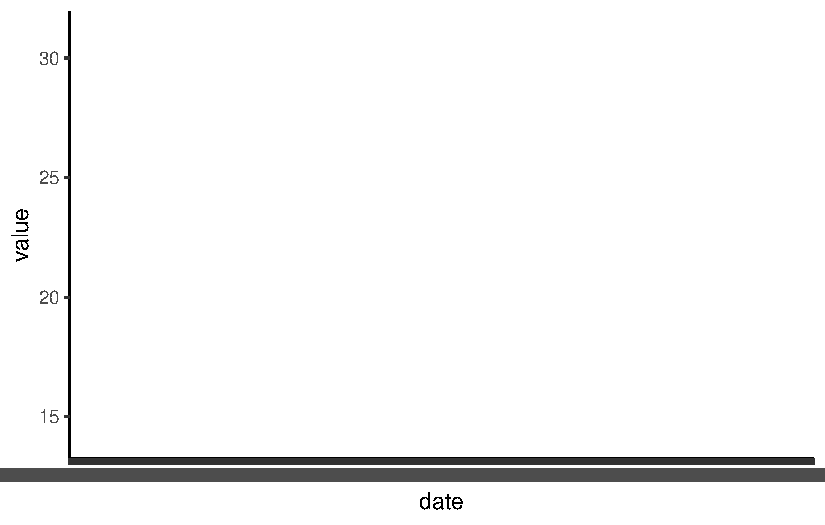
\includegraphics{datetime_files/figure-pdf/unnamed-chunk-4-1.pdf}

\textbf{same graph after making date into a date/time object}

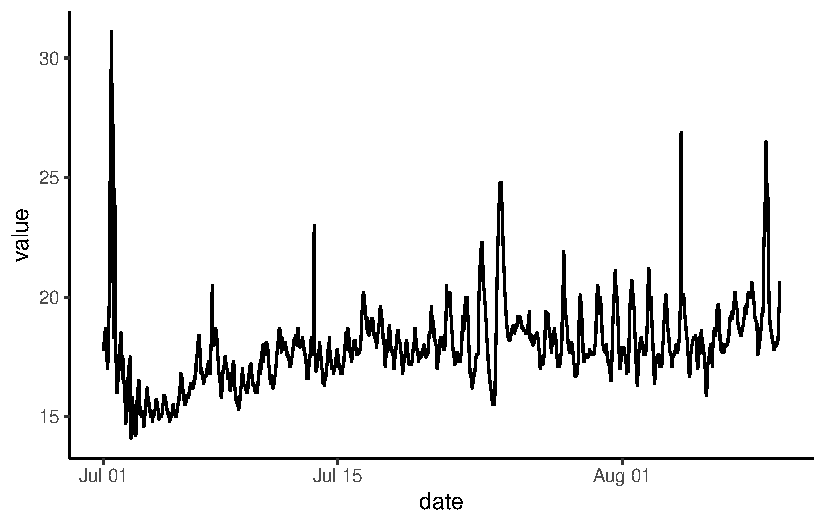
\includegraphics{datetime_files/figure-pdf/unnamed-chunk-5-1.pdf}

\begin{center}\rule{0.5\linewidth}{0.5pt}\end{center}



\end{document}
